\subsection{Normalización de la Base de Datos}
Para asegurar que la información no se repita, no ocupe espacio de más y no cause errores al guardar o borrar registros, se aplicó el proceso de normalización hasta la Tercera Forma Normal (3FN). En palabras sencillas, normalizar es como ordenar una habitación: consiste en repartir los datos en cajones o tablas independientes para que cada dato esté exactamente en el lugar que le corresponde.

\subsubsection{Primera Forma Normal (1FN): Datos atómicos y sin listas repetidas}
La regla de la Primera Forma Normal pide que cada campo o columna guarde un solo dato elemental (que sea indivisible o atómico) y que no existan listas o grupos repetidos dentro de una misma celda.

En este nuevo diseño se aplicó lo siguiente:
\begin{itemize}
    \item \textbf{Separación de nombres:} En lugar de guardar el nombre completo en un solo texto largo, se dividió en campos individuales: \texttt{primer\_nombre}, \texttt{segundo\_nombre}, \texttt{apellido\_paterno} y \texttt{apellido\_materno} dentro de la tabla \texttt{persona}.
    \item \textbf{Extracción de teléfonos y correos repetidos:} Una persona puede tener más de un número telefónico o varios correos. Si se guardaran en la misma fila separados por comas, se violaría la 1FN. Por ello, se crearon las tablas independientes \texttt{telefono} (con \texttt{numero}, \texttt{extension} y \texttt{region}) y \texttt{email} (con \texttt{direccion\_email} y la marca \texttt{es\_principal}), cada una conectada a su dueño mediante una llave foránea.
\end{itemize}

\subsubsection{Segunda Forma Normal (2FN): Dependencia funcional completa}
La Segunda Forma Normal exige que la tabla ya cumpla con la 1FN y que todos los datos que no son llaves dependan por completo de la llave principal, no solo de un pedazo de ella (aplica especialmente en tablas con llaves compuestas).

En el modelo se cuidó esta regla en las siguientes tablas dependientes:
\begin{itemize}
    \item \textbf{Tabla \texttt{entregable\_version}:} Cada entrega se identifica por el proyecto y el número de versión. Datos como la ruta del archivo PDF, la fecha de subida, los comentarios del alumno y las observaciones del maestro dependen enteramente de esa entrega específica y no solo del proyecto general.
    \item \textbf{Tabla \texttt{compromiso\_acuerdo}:} Cada tarea depende de la minuta en la que se acordó y del número de tarea asignado. La descripción de la tarea, el responsable, la fecha límite y el estado de cumplimiento dependen de esa tarea puntual.
\end{itemize}

\subsubsection{Tercera Forma Normal (3FN): Eliminar dependencias transitivas}
La Tercera Forma Normal establece que la tabla ya esté en 2FN y que ningún dato dependa de otro dato que no sea la llave principal (es decir, evitar depender de datos intermedios o dependencias transitivas).

En el nuevo diseño se solucionó esto separando responsabilidades:
\begin{itemize}
    \item \textbf{Separación de Persona, Cuenta y Rol:} Se separó la información de la persona física (nombre y apellidos) de sus credenciales de acceso al sistema (tabla \texttt{cuenta}, con \texttt{contrasena}, \texttt{fecha\_registro} y \texttt{cuenta\_activa}). A su vez, el tipo de usuario o rol no se dejó como un texto suelto en la cuenta, sino que se extrajo a la tabla \texttt{rol} (\texttt{id\_rol}, \texttt{nombre\_tipo}). De esta forma, si cambia el nombre de un rol o los permisos, no se altera la tabla de cuentas ni la de personas.
    \item \textbf{Separación de Proyectos y Alertas:} La tabla \texttt{alerta\_rezago} guarda de forma independiente la fecha de detección, los días acumulados y el estado del aviso, dependiendo directamente de su propio identificador (\texttt{id\_alerta}) y enlazándose al proyecto únicamente mediante su llave foránea.
\end{itemize}

En la Figura~\ref{fig:er_normalizado} se muestra el diagrama Entidad--Relación obtenido tras aplicar las tres formas normales, detallando las entidades resultantes, sus atributos elementales y las llaves primarias identificadoras.

\begin{figure}[htbp]
    \centering
    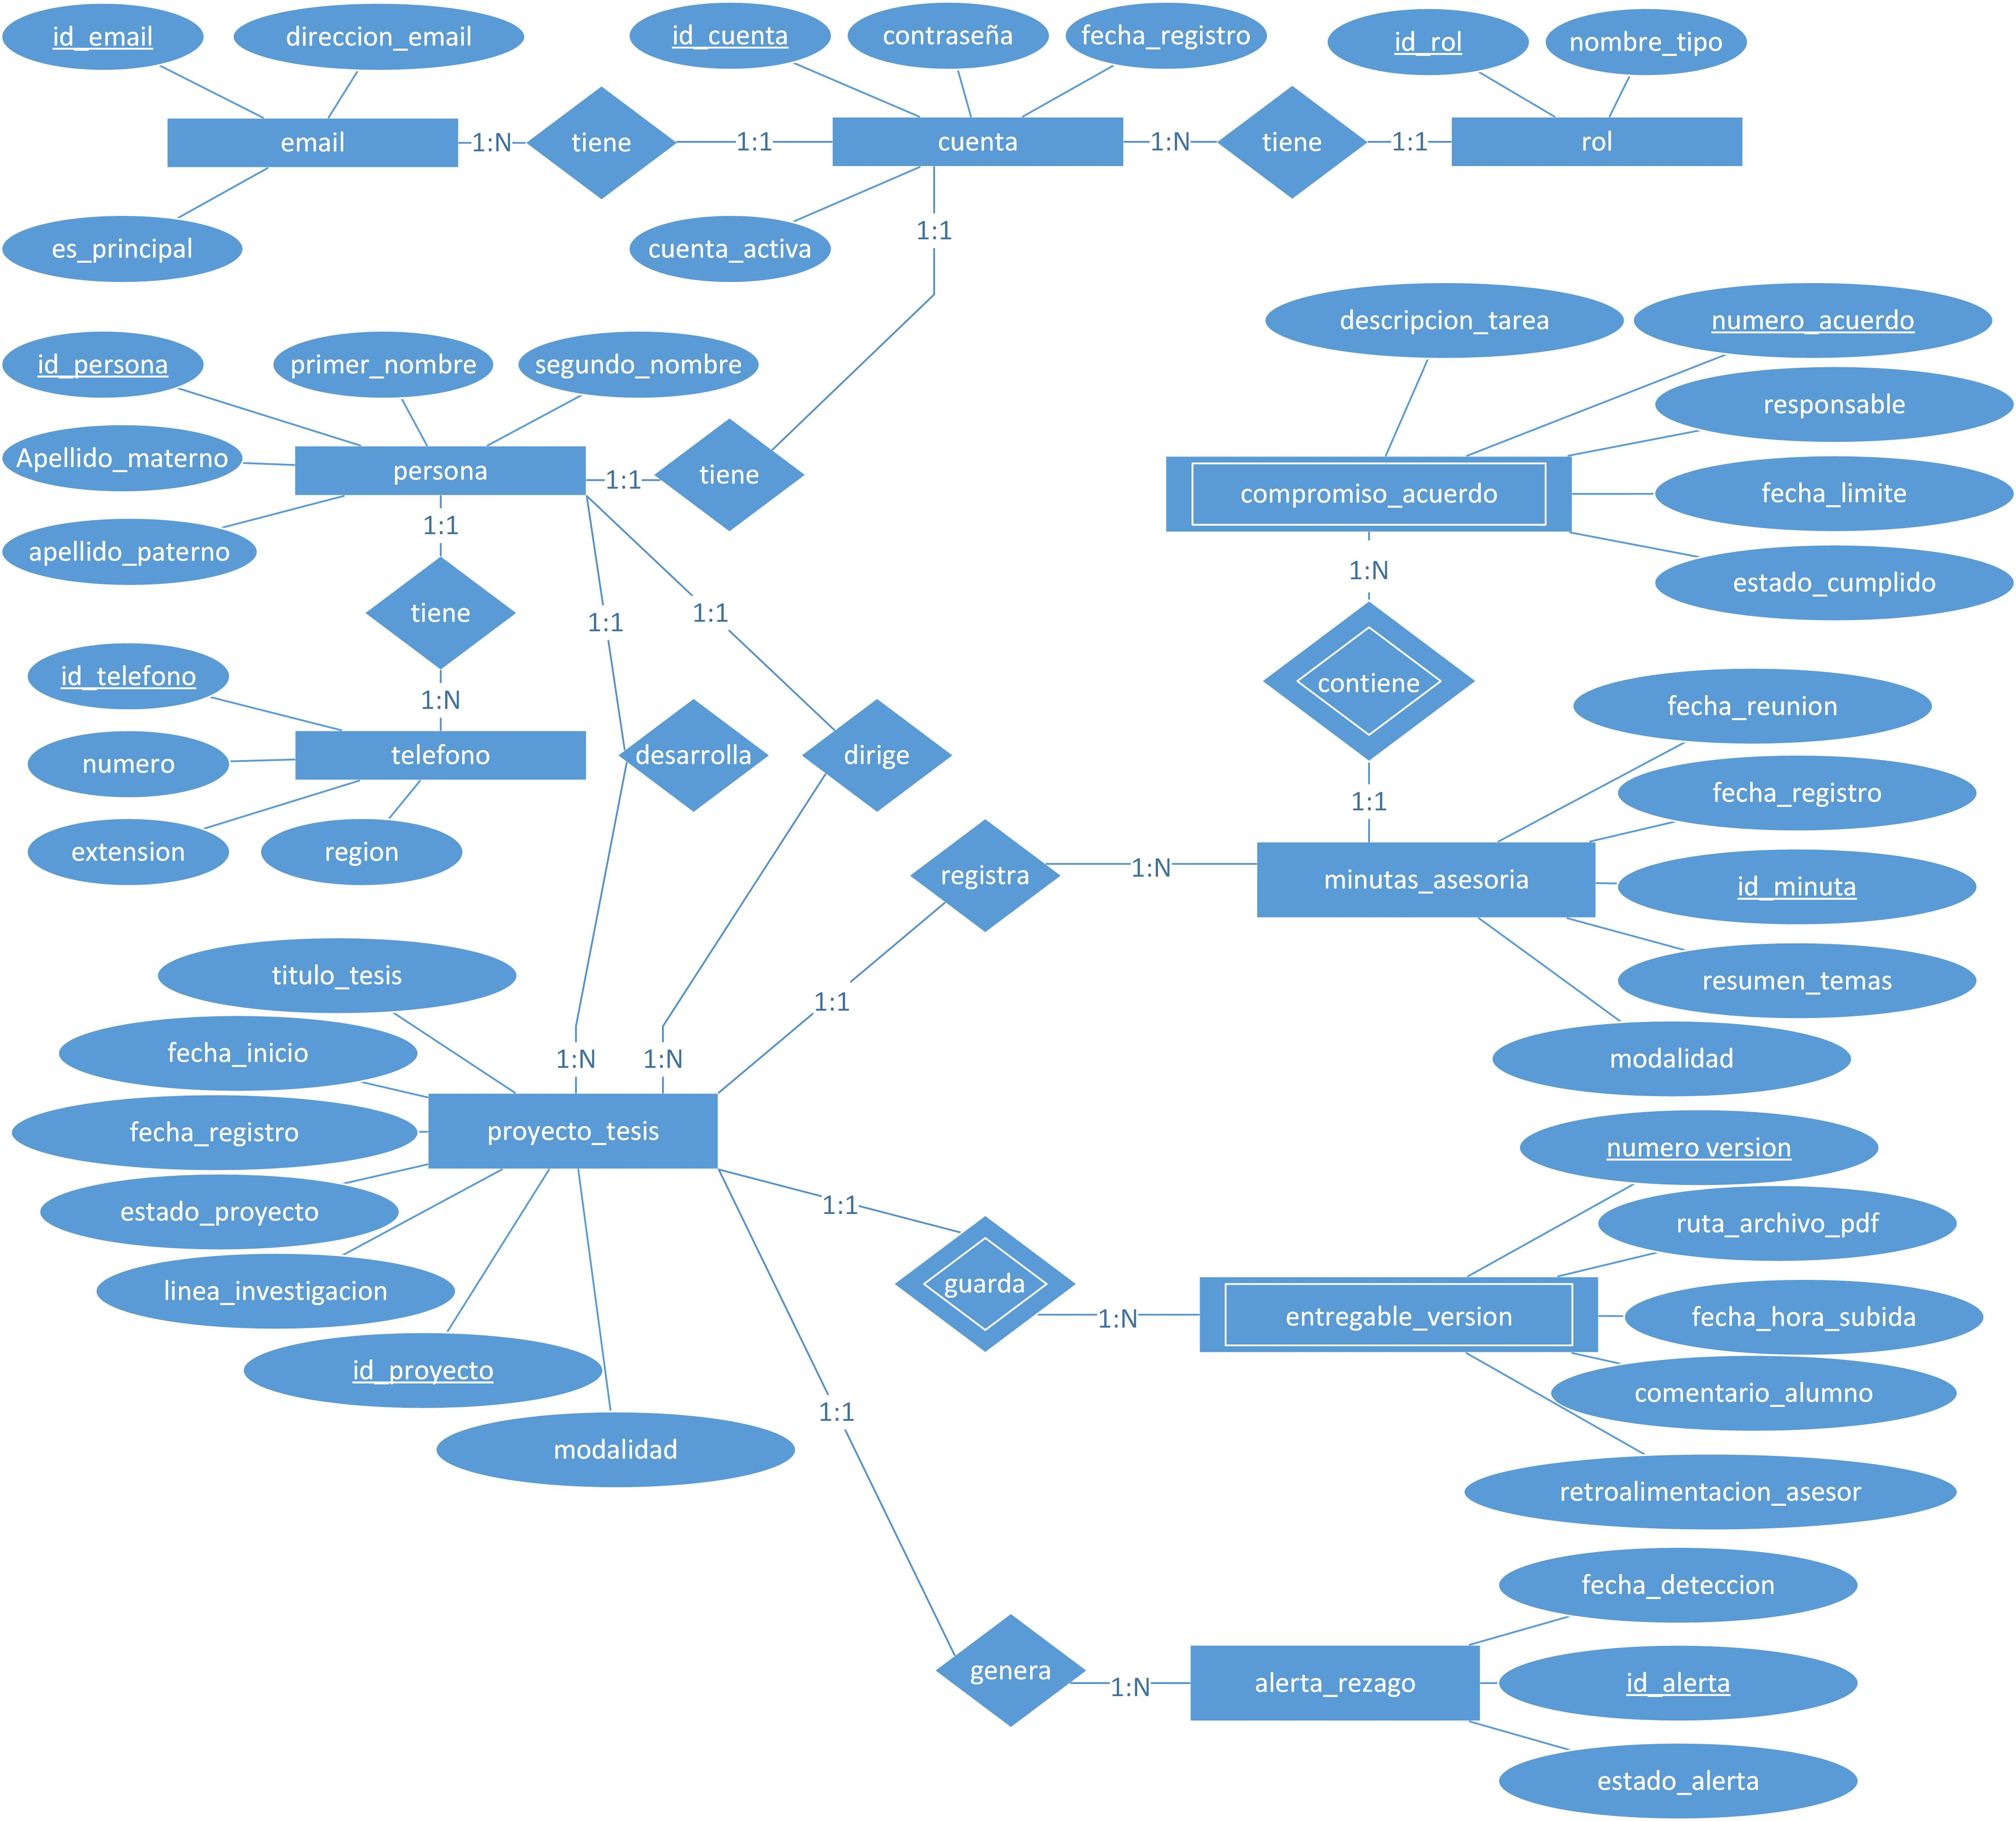
\includegraphics[width=0.95\textwidth]{assets/database/db-MER-FN3.jpg}
    \caption{Diagrama Entidad--Relación normalizado en Tercera Forma Normal (3FN).}
    \label{fig:er_normalizado}
\end{figure}